% !TEX program = pdflatex
\documentclass[a4paper,12pt]{article}

% ── Pakiety ──────────────────────────────────────────────────
\usepackage[utf8]{inputenc}
\usepackage[T1]{fontenc}
\usepackage{polski}
\usepackage[english]{babel}
\usepackage[margin=2.2cm]{geometry}
\usepackage{amsmath}
\usepackage{hyperref}
\usepackage{xcolor}
\usepackage{tikz}
\usetikzlibrary{shapes.geometric,arrows.meta,positioning,calc,fit,
                backgrounds,shadows,decorations.pathreplacing,
                matrix,chains,scopes}
\usepackage{tcolorbox}
\tcbuselibrary{skins,breakable}
\usepackage{listings}
\usepackage{fontawesome5}
\setlength{\headheight}{27pt}
\usepackage{fancyhdr}
\usepackage{tocloft}
\usepackage{enumitem}
\usepackage{tabularx}
\usepackage{booktabs}
\usepackage{colortbl}
\usepackage{array}
\usepackage{multirow}
\usepackage{fancyvrb}
\usepackage{needspace}
\usepackage{parskip}

% ── Kolory cyberpunk ─────────────────────────────────────────
\definecolor{bg}{HTML}{0a0e17}
\definecolor{fg}{HTML}{c0c0c0}
\definecolor{accent}{HTML}{00ffaa}
\definecolor{pink}{HTML}{ff66cc}
\definecolor{red}{HTML}{e94560}
\definecolor{orange}{HTML}{ffaa00}
\definecolor{darkbg}{HTML}{1a1a2e}
\definecolor{mediumbg}{HTML}{161b22}
\definecolor{border}{HTML}{2a2a3c}

% ── Konfiguracja listings ────────────────────────────────────
\lstdefinestyle{cppstyle}{
    backgroundcolor=\color{darkbg},
    commentstyle=\color{orange},
    keywordstyle=\color{pink}\bfseries,
    stringstyle=\color{accent},
    basicstyle=\ttfamily\footnotesize\color{fg},
    breaklines=true,
    frame=single,
    framerule=0.5pt,
    rulecolor=\color{red},
    numbers=left,
    numberstyle=\tiny\color{fg!50},
    numbersep=8pt,
    tabsize=4,
    showstringspaces=false,
    captionpos=b,
    aboveskip=8pt,
    belowskip=8pt,
}

\lstdefinestyle{luastyle}{
    backgroundcolor=\color{darkbg},
    commentstyle=\color{orange},
    keywordstyle=\color{pink}\bfseries,
    stringstyle=\color{accent},
    basicstyle=\ttfamily\footnotesize\color{fg},
    breaklines=true,
    frame=single,
    framerule=0.5pt,
    rulecolor=\color{red},
    numbers=left,
    numberstyle=\tiny\color{fg!50},
    numbersep=8pt,
    tabsize=2,
    showstringspaces=false,
    captionpos=b,
    aboveskip=8pt,
    belowskip=8pt,
}

\lstdefinestyle{jsonstyle}{
    backgroundcolor=\color{darkbg},
    stringstyle=\color{accent},
    basicstyle=\ttfamily\footnotesize\color{fg},
    breaklines=true,
    frame=single,
    framerule=0.5pt,
    rulecolor=\color{red},
    tabsize=2,
    showstringspaces=false,
}

\lstdefinestyle{bashstyle}{
    backgroundcolor=\color{darkbg},
    basicstyle=\ttfamily\footnotesize\color{accent},
    breaklines=true,
    frame=single,
    framerule=0.5pt,
    rulecolor=\color{red},
}

% ── Tcolorbox style ──────────────────────────────────────────
\newtcolorbox{infobox}[1][]{
    colback=darkbg,
    colframe=red,
    coltitle=fg,
    fonttitle=\bfseries,
    title=#1,
    arc=4pt,
    boxrule=1pt,
    before skip=10pt,
    after skip=10pt,
}

\newtcolorbox{warnbox}{
    colback=darkbg,
    colframe=orange,
    arc=4pt,
    boxrule=1pt,
    before skip=10pt,
    after skip=10pt,
}

% ── Nagłówki / stopki ────────────────────────────────────────
\pagestyle{fancy}
\fancyhf{}
\fancyhead[L]{\textcolor{accent}{\textbf{MagistralaCAN4}}}
\fancyhead[R]{\textcolor{pink}{Dokumentacja techniczna}}
\fancyfoot[C]{\textcolor{fg!50}{\thepage}}
\renewcommand{\headrulewidth}{1pt}
\renewcommand{\headrule}{\hbox to\headwidth{\color{red}\leaders\hrule height \headrulewidth\hfill}}

% ── TOC styling ──────────────────────────────────────────────
\renewcommand{\cftsecfont}{\color{accent}\bfseries}
\renewcommand{\cftsubsecfont}{\color{pink}}
\renewcommand{\cftsubsubsecfont}{\color{orange}}
\renewcommand{\cftsecpagefont}{\color{accent}}
\renewcommand{\cftsubsecpagefont}{\color{pink}}

% ── Hiperłącza ───────────────────────────────────────────────
\hypersetup{
    colorlinks=true,
    linkcolor=accent,
    urlcolor=pink,
    citecolor=orange,
}

% ── Tytuł ────────────────────────────────────────────────────
\title{
    \vspace{-2cm}
    {\Huge\color{accent}\textbf{MagistralaCAN4}}\\[8pt]
    {\Large\color{pink}Wysokowydajny sniffer CAN / CAN FD}\\[4pt]
    {\normalsize\color{fg}Uczenie asocjacyjne \,\textbullet{} \, Silnik Lua \,\textbullet{} \, Akceleracja GPU \,\textbullet{} \, WebSocket}\\[12pt]
    {\small\color{orange}Wersja 2.0.0 \,|\, C++17 \,|\, Qt\,6.10 \,|\, Linux socketCAN}
}
\author{\color{fg}CustomLabs}
\date{\color{fg}\today}

\begin{document}
\maketitle
\thispagestyle{empty}

\begin{tikzpicture}[overlay,remember picture]
    \draw[red,line width=1.5pt]
        ([shift={(-1cm,0.5cm)}]current page.south west) --
        ([shift={(1cm,0.5cm)}]current page.south east);
    \draw[accent,line width=0.5pt]
        ([shift={(-1cm,0.2cm)}]current page.south west) --
        ([shift={(1cm,0.2cm)}]current page.south east);
\end{tikzpicture}

\vfill
\begin{center}
    \color{fg!70}\footnotesize
    \faLinux\ Linux (Kali) \quad\faMicrochip\ socketCAN \quad\faCode\ C++17/Qt6 \quad\faCogs\ OpenCL
\end{center}

\newpage
\tableofcontents
\newpage

% ═══════════════════════════════════════════════════════════════
\section{Schemat blokowy}
% ═══════════════════════════════════════════════════════════════

\begin{figure}[h!]
\centering
\begin{tikzpicture}[
    node distance=8mm and 12mm,
    block/.style={
        rectangle, draw=red, fill=darkbg, text=fg,
        rounded corners=3pt, minimum width=2.4cm, minimum height=0.8cm,
        align=center, font=\footnotesize, line width=0.8pt,
        drop shadow={shadow xshift=1.5pt, shadow yshift=-1.5pt, fill=red!40}
    },
    coreblock/.style={
        rectangle, draw=accent, fill=darkbg, text=accent,
        rounded corners=3pt, minimum width=2.6cm, minimum height=0.8cm,
        align=center, font=\footnotesize\bfseries, line width=0.8pt,
    },
    guiblock/.style={
        rectangle, draw=pink, fill=darkbg, text=pink,
        rounded corners=3pt, minimum width=2.8cm, minimum height=0.8cm,
        align=center, font=\footnotesize, line width=0.8pt,
    },
    outblock/.style={
        rectangle, draw=orange, fill=darkbg, text=orange,
        rounded corners=3pt, minimum width=2.4cm, minimum height=0.7cm,
        align=center, font=\footnotesize, line width=0.8pt,
    },
    group/.style={
        rectangle, draw=border, fill=mediumbg!30,
        rounded corners=6pt, inner sep=10pt, line width=1.2pt, dashed,
    },
    arrow/.style={->, >=Stealth, line width=0.7pt, color=fg!60},
    label/.style={font=\tiny\color{fg!70}, align=center},
]

% Węzły
\node[coreblock] (sock) at (0,2.2) {socketCAN\\\scriptsize vcan0 / can0};

\node[coreblock] (sniffer) at (0,1.0) {CanSniffer\\\scriptsize odczyt/wątki};

\node[coreblock] (model) at (-2.5,-0.4) {CanFrameModel\\\scriptsize batch 33ms};
\node[coreblock] (lua) at (0,-0.4) {LuaScriptEngine\\\scriptsize Lua 5.4};
\node[coreblock] (dbc) at (2.5,-0.4) {DbcParser\\\scriptsize pliki .dbc};

\node[coreblock] (learn) at (-2.5,-1.8) {AssociativeLearner\\\scriptsize analityka};
\node[coreblock] (gpu) at (0,-1.8) {GpuCorrelator\\\scriptsize OpenCL};
\node[coreblock] (ws) at (2.5,-1.8) {WebSocketServer\\\scriptsize port 9000};

% GUI
\node[guiblock] (tabcan) at (7.5,1.5) {Ruch CAN};
\node[guiblock] (tablearn) at (7.5,0.5) {Uczenie asoc.};
\node[guiblock] (tabdet) at (7.5,-0.5) {Szczegóły ramki};
\node[guiblock] (taboff) at (7.5,-1.5) {Analiza offline};
\node[guiblock] (tabdash) at (7.5,-2.5) {Dashboard CAN};

% Output
\node[outblock] (tray) at (12.5,0.3) {System tray};
\node[outblock] (log) at (12.5,-0.6) {Logger};
\node[outblock] (wsout) at (12.5,-1.5) {WebSocket clients};

% Połączenia
\draw[arrow] (sock) -- (sniffer);
\draw[arrow] (sniffer.south) -- ++(0,-0.15) -| (model.north);
\draw[arrow] (sniffer.south) -- ++(0,-0.15) -| (lua.north);
\draw[arrow] (sniffer.south) -- ++(0,-0.15) -| (dbc.north);
\draw[arrow] (sniffer) -- (learn);

\draw[arrow] (model) -- (tabcan);
\draw[arrow] (lua) to[bend left=20] (sniffer);
\draw[arrow] (learn) -- (tablearn);
\draw[arrow] (dbc) -- (tabdet);
\draw[arrow] (dbc) -- (tabdash);

\draw[arrow] (model) -- (ws);
\draw[arrow] (learn) -- (gpu);

\draw[arrow] (ws) -- (wsout);
\draw[arrow] (learn) to[bend right=30] (tray);
\draw[arrow] (learn) to[bend right=30] (log);

% Grupy – rysowane jako tła
\begin{scope}[on background layer]
    \node[group, fit=(sock), inner sep=8pt,
          label={[accent]north:{\textbf{Warstwa sprzętowa}}}] (hw) {};
    \node[group, fit=(sniffer)(model)(lua)(dbc)(learn)(gpu)(ws), inner sep=10pt,
          label={[accent]north:{\textbf{Rdzeń (C++17 / Qt6)}}}] (core) {};
    \node[group, fit=(tabcan)(tablearn)(tabdet)(taboff)(tabdash), inner sep=10pt,
          label={[pink]north:{\textbf{Interfejs użytkownika}}}] (gui) {};
    \node[group, fit=(tray)(log)(wsout), inner sep=10pt,
          label={[orange]north:{\textbf{Wyjście}}}] (out) {};
\end{scope}

\end{tikzpicture}
\caption{Schemat blokowy architektury MagistralaCAN4}
\label{fig:block}
\end{figure}

% ═══════════════════════════════════════════════════════════════
\section{Wprowadzenie}
% ═══════════════════════════════════════════════════════════════

\textbf{MagistralaCAN4} to zaawansowane narzędzie do analizy magistrali CAN, zaprojektowane z myślą o inżynierach motoryzacyjnych, badaczach systemów wbudowanych i entuzjastach reverse engineeringu protokołów komunikacyjnych. Aplikacja łączy przechwytywanie ruchu CAN w czasie rzeczywistym z zaawansowaną analityką danych, uczeniem asocjacyjnym i zdalnym dostępem przez WebSocket.

\begin{infobox}[Kluczowe cechy]
\begin{itemize}[nosep]
    \item Wielowątkowy odczyt CAN/CAN FD przez socketCAN
    \item Zaawansowane uczenie asocjacyjne (14 tabel analitycznych, klastrowanie, PCA, anomalie)
    \item Silnik skryptowy Lua z API CAN (sendFrame, log, getTick)
    \item Akceleracja GPU przez OpenCL (fallback CPU)
    \item Serwer WebSocket streamujący ramki jako JSON
    \item Parser DBC z integracją sygnałów w dashboardzie
    \item Analiza offline plików candump
    \item Interaktywny edytor ramek z siatką bitów
\end{itemize}
\end{infobox}

% ═══════════════════════════════════════════════════════════════
\section{Architektura systemu}
% ═══════════════════════════════════════════════════════════════

\subsection{Przepływ ramki CAN}

Poniższy diagram sekwencji przedstawia drogę ramki od socketCAN przez wszystkie warstwy systemu:

\begin{center}
\begin{tikzpicture}[
    box/.style={rectangle, draw=accent, fill=darkbg, text=fg,
                minimum width=2.8cm, minimum height=0.7cm, align=center,
                font=\footnotesize, rounded corners=2pt},
    arrow/.style={->, >=Stealth, line width=0.8pt, color=red},
    time/.style={font=\tiny\color{fg!50}},
]

\node[box,draw=red] (socket) {socketCAN\\read()};
\node[box,right=of socket] (snif) {CanSniffer\\doWork()};
\node[box,right=of snif] (parse) {parseFrame()};
\node[box,right=of parse] (emit) {emit newFrame};

\node[box,draw=pink,below=1.5cm of emit,xshift=-3.2cm] (gui) {MainWindow\\onNewFrame};
\node[box,draw=pink,below=1.5cm of emit] (learn) {Associative\\Learner};
\node[box,draw=pink,below=1.5cm of emit,xshift=3.2cm] (luaeng) {LuaScript\\Engine};

\node[box,draw=orange,below=of gui] (model) {CanFrameModel\\33ms batch};
\node[box,draw=orange,below=of model] (table) {QTableView\\Ruch CAN};

\draw[arrow] (socket) -- (snif);
\draw[arrow] (snif) -- (parse);
\draw[arrow] (parse) -- (emit);
\draw[arrow] (emit) |- (gui);
\draw[arrow] (emit) -- (learn);
\draw[arrow] (emit) |- (luaeng);
\draw[arrow] (gui) -- (model);
\draw[arrow] (model) -- (table);

\end{tikzpicture}
\end{center}

\subsection{Komponenty rdzenia}

\begin{tabularx}{\textwidth}{@{}>{\color{accent}\bfseries}lX@{}}
\toprule
\rowcolor{darkbg} Komponent & Odpowiedzialność \\
\midrule
CanSniffer & Wielowątkowy odczyt/zapis socketCAN (QtConcurrent::run). Emituje sygnał \texttt{newFrame} dla każdej ramki. \\
CanFrameModel & QAbstractTableModel z 6 kolumnami. Nadpisywanie wg ID, aktualizacja wsadowa co 33 ms. \\
AssociativeLearner & Uczenie asocjacyjne, korelacje, klastrowanie, anomalie, predykcja. \\
LuaScriptEngine & Interpreter Lua 5.4 z API CAN: \texttt{sendFrame}, \texttt{log}, \texttt{getTick}. \\
DbcParser & Parsowanie plików \texttt{.dbc}, dekompozycja sygnałów. \\
GpuCorrelator & Obliczenia macierzy podobieństw na GPU (OpenCL) lub CPU. \\
WebSocketServer & Serwer WebSocket na porcie 9000, stream JSON ramek CAN. \\
Logger & Zapis zdarzeń do \texttt{\textasciitilde/magistrala\_can4.log}. \\
\bottomrule
\end{tabularx}

% ═══════════════════════════════════════════════════════════════
\section{Zakładki aplikacji}
% ═══════════════════════════════════════════════════════════════

\subsection{Ruch CAN}

Główna tabela pokazująca ruch na magistrali w czasie rzeczywistym. Zawiera 6 kolumn: ID, Extended, RTR, DLC, Data (szesnastkowo), Timestamp. Checkbox \texttt{Nadpisywanie} w toolbarze kontroluje, czy nowsze ramki o tym samym ID zastępują starsze. Przycisk \texttt{Eksportuj candump} zapisuje bieżący stan tabeli do pliku w standardowym formacie candump.

\subsection{Szczegóły ramki}

Widok pojedynczej ramki CAN (po kliknięciu w tabeli). Zawiera:

\begin{itemize}[nosep]
    \item \textbf{Siatkę bitów 8$\times$8} — każdy bajt jest wizualizowany jako 8 bitów (0/1)
    \item \textbf{Podświetlanie zmian} — bity zmienione względem poprzedniej ramki tego samego ID
    \item \textbf{Sygnały DBC} — po wczytaniu pliku .dbc pokazuje nazwy i wartości sygnałów
    \item \textbf{Edycję ramek} — kliknięcie bajtu umożliwia edycję (hex lub przełączanie bitów)
    \item \textbf{Wysyłanie} — przycisk \texttt{Wyślij zmodyfikowaną ramkę}
\end{itemize}

\subsection{Analiza offline}

Odtwarzacz plików candump:

\begin{itemize}[nosep]
    \item Wczytywanie standardowych plików candump
    \item Suwak prędkości: od 0.1$\times$ do 10$\times$ prędkości oryginalnej
    \item Tryb oryginalnych timestampów lub stałego interwału
    \item Tryb krokowy: przycisk \texttt{Następna ramka} / klawisz \texttt{Enter}
    \item Integracja z AssociativeLearner i LuaScriptEngine
\end{itemize}

\subsection{Dashboard CAN}

Dashboard sygnałów DBC aktualizowany na żywo. Po wczytaniu pliku .dbc automatycznie tworzy panele (QLabel) dla wszystkich sygnałów, wyświetlając nazwę, aktualną wartość i jednostkę.

% ═══════════════════════════════════════════════════════════════
\section{Uczenie asocjacyjne — szczegółowy opis}
% ═══════════════════════════════════════════════════════════════

\subsection{Filozofia działania}

System uczy się powiązań między \textbf{zmiennymi użytkownika} (np. temperatura, prędkość obrotowa) a \textbf{ramkami CAN}. Użytkownik rejestruje zdarzenia (wartość zmiennej + okno czasowe ramek CAN), a system znajduje identyfikatory CAN, których charakterystyka koreluje ze zmianami zmiennej. Dodatkowo można rejestrować \textbf{braki zdarzeń} jako tło kontrastowe, które obniża score kandydatów podobnych do tła.

\begin{figure}[h!]
\centering
\begin{tikzpicture}[
    phase/.style={rectangle, draw=accent, fill=darkbg, text=fg,
                  rounded corners=4pt, minimum width=3cm, minimum height=1cm,
                  align=center, font=\small, line width=1pt},
    arrow/.style={->, >=Stealth, line width=1pt, color=red},
]

\node[phase,draw=orange] (user) {Użytkownik\\rejestruje zdarzenia};
\node[phase,right=of user] (extract) {Ekstrakcja\\wektorów cech};
\node[phase,right=of extract] (sim) {Obliczanie\\podobieństwa};
\node[phase,below=of sim] (rank) {Ranking\\kandydatów};
\node[phase,left=of rank] (contrast) {Kontrast\\z tłem};

\draw[arrow] (user) -- (extract);
\draw[arrow] (extract) -- (sim);
\draw[arrow] (sim) -- (rank);
\draw[arrow] (rank) -- (contrast);
\draw[arrow] (contrast) -- (user);

\node[font=\footnotesize\color{orange},below=0.3cm of contrast] {non‑eventy obniżają score};
\end{tikzpicture}
\caption{Cykl uczenia asocjacyjnego}
\label{fig:learncycle}
\end{figure}

\subsection{Wektor cech}

Dla każdego ID w oknie zdarzenia budowany jest 67-elementowy wektor cech:

\begin{tikzpicture}[
    feat/.style={rectangle, draw=border, fill=darkbg, text=fg,
                 minimum width=1.8cm, minimum height=0.6cm,
                 font=\tiny, align=center},
]

\node[feat,draw=accent] (f0) {$f_0$: liczba\\ramek};
\node[feat,right=0pt of f0] (f1) {$f_1$: śr.\\odstęp};
\node[feat,right=0pt of f1] (f2) {$f_2$: odch.\\stand.};
\node[feat,right=0pt of f2,draw=pink] (f3) {$f_{3\dots66}$: śr. bajtów\\64 bajty / 255};

\node[font=\footnotesize\color{fg!60},above=0.2cm of f0] {3 cechy statystyczne};
\node[font=\footnotesize\color{pink},above=0.2cm of f3] {64 cechy sygnałowe};
\end{tikzpicture}

\subsection{Miara podobieństwa}

Podobieństwo między dwoma wektorami cech $v_1$, $v_2$ obliczane jest jako podobieństwo cosinusowe:

\[
\operatorname{sim}(v_1, v_2) = \frac{v_1 \cdot v_2}{\|v_1\|_2 \cdot \|v_2\|_2 + \varepsilon}
\]

gdzie $\varepsilon = 10^{-6}$ zapobiega dzieleniu przez zero.

\subsection{Tabele analityczne}

\begin{center}
\begin{tikzpicture}[
    tablebox/.style={rectangle, draw=red, fill=darkbg, text=fg,
                     rounded corners=3pt, minimum width=3.8cm, minimum height=0.8cm,
                     align=center, font=\footnotesize,
                     drop shadow={shadow xshift=1pt, shadow yshift=-1pt, fill=red!30}},
]

\node[tablebox,draw=accent] (corr) {Korelacja\\wartość--bajt};
\node[tablebox,right=of corr] (seq) {Sekwencje\\bigram/trigram};
\node[tablebox,right=of seq] (cross) {Korelacja\\międzybajtowa};

\node[tablebox,draw=orange,below=of corr] (mi) {Mutual\\Information};
\node[tablebox,draw=orange,below=of seq] (mic) {MIC\\(max 8$\times$8)};
\node[tablebox,draw=orange,below=of cross] (pred) {Predykcja\\regresja liniowa};

\node[tablebox,draw=pink,below=of mi] (markov) {Predykcja\\Markowa};
\node[tablebox,draw=pink,below=of mic] (cluster) {Klastrowanie\\k-średnich};
\node[tablebox,draw=pink,below=of pred] (anom) {Detekcja\\anomalii};

\end{tikzpicture}
\end{center}

% Mini opis każdej tabeli
\begin{itemize}[nosep]
    \item \textbf{Korelacja wartość--bajt} — Pearson $r$ między zmienną a bajtami
    \item \textbf{Sekwencje} — najczęstsze sekwencje ID (bigramy/trigramy)
    \item \textbf{Korelacja międzybajtowa} — Pearson $r$ między parami bajtów
    \item \textbf{Mutual Information} — zależności nieliniowe (histogram 10$\times$10, zrównoleglony)
    \item \textbf{MIC} — Maximal Information Coefficient (siatki 2$\times$2 do 8$\times$8)
    \item \textbf{Predykcja wartości} — regresja $y = a\cdot\mathrm{byte} + b$, tylko $|r| > 0.8$
    \item \textbf{Markov} — najbardziej prawdopodobny następny ID
    \item \textbf{Klastrowanie} — k-średnich, auto-K (łokieć), PCA+2D
    \item \textbf{Anomalie} — model normalny, Z-score, próg konfigurowalny
\end{itemize}

\subsection{Klastrowanie}

Moduł klastrowania grupuje okna czasowe w 3 klastry na podstawie 5-wymiarowych wektorów cech: liczby ramek, liczby unikalnych ID, entropii rozkładu ID oraz czasu trwania okna. Dodatkowo dostępne są:

\begin{itemize}[nosep]
    \item \textbf{Auto K (łokieć)} — automatyczny dobór optymalnej liczby klastrów metodą łokcia (WCSS)
    \item \textbf{PCA + k-średnich} — redukcja do 2D metodą potęgową, wizualizacja scatter plot
\end{itemize}

\subsection{Eksport i import}

\begin{center}
\begin{tikzpicture}[
    export/.style={rectangle, draw=accent, fill=darkbg, text=fg,
                   rounded corners=3pt, minimum width=3.2cm, minimum height=0.7cm,
                   align=center, font=\footnotesize},
    arrow/.style={<->, >=Stealth, line width=0.8pt, color=orange},
]

\node[export] (session) {Sesja (JSON)};
\node[export,right=0.5cm of session] (models) {Modele (JSON)};
\node[export,right=0.5cm of models] (luaexp) {Skrypt Lua};
\node[export,right=0.5cm of luaexp] (html) {Raport HTML};

\node[font=\footnotesize\color{fg!60},below=0.3cm of session] {pełny stan};
\node[font=\footnotesize\color{fg!60},below=0.3cm of models] {transfer learning};
\node[font=\footnotesize\color{fg!60},below=0.3cm of luaexp] {top‑5 reguł};
\node[font=\footnotesize\color{fg!60},below=0.3cm of html] {wszystkie tabele};

\end{tikzpicture}
\end{center}

% ═══════════════════════════════════════════════════════════════
\section{Silnik skryptowy Lua}
% ═══════════════════════════════════════════════════════════════

Silnik Lua 5.4 jest zintegrowany przez \texttt{LuaScriptEngine}. Skrypty są ładowane w toolbarze (\texttt{Wczytaj skrypt Lua}). Każda ramka CAN wyzwala funkcję \texttt{onFrame(id, data, timestamp)}.

\subsection{API}

\begin{tcolorbox}[colback=darkbg, colframe=accent, title={\color{accent}\textbf{sendFrame(id, data\_table)}}, arc=4pt]
Wysyła ramkę CAN na magistralę.\\
\textbf{Parametry}: \texttt{id} (integer), \texttt{data\_table} (tabela bajtów, indeksowana od 1, maks. 64).\\
\textbf{Zwraca}: \texttt{true} lub \texttt{false, error\_msg}.
\begin{lstlisting}[style=luastyle, frame=none, backgroundcolor=\color{darkbg}]
local ok, err = sendFrame(0x123, {0xAA, 0xBB, 0xCC})
if not ok then log("Blad: " .. err) end
\end{lstlisting}
\end{tcolorbox}

\begin{tcolorbox}[colback=darkbg, colframe=pink, title={\color{pink}\textbf{log(message)}}, arc=4pt]
Zapisuje wiadomość do logu (\texttt{\textasciitilde/magistrala\_can4.log}).
\begin{lstlisting}[style=luastyle, frame=none, backgroundcolor=\color{darkbg}]
log("Odebrano ramke ID: " .. string.format("0x%X", id))
\end{lstlisting}
\end{tcolorbox}

\begin{tcolorbox}[colback=darkbg, colframe=orange, title={\color{orange}\textbf{getTick()}}, arc=4pt]
Zwraca liczbę milisekund od uruchomienia silnika Lua.
\begin{lstlisting}[style=luastyle, frame=none, backgroundcolor=\color{darkbg}]
local uptime_ms = getTick()
\end{lstlisting}
\end{tcolorbox}

\subsection{Pełny przykład}

\begin{lstlisting}[style=luastyle, caption={Monitorowanie ID 0x123 z automatyczną odpowiedzią}]
function onFrame(id, data, timestamp)
    if id == 0x123 then
        if data[1] > 0x80 then
            log("Wysoka wartosc: " .. data[1])
            sendFrame(0x456, {0x01, 0x02})
        end
    end
end
\end{lstlisting}

\subsection{Generowanie skryptów z uczenia asocjacyjnego}

Przycisk \texttt{Generuj skrypt Lua} automatycznie tworzy skrypt z regułami dla top-5 kandydatów:

\begin{lstlisting}[style=luastyle, caption={Automatycznie wygenerowany skrypt}]
-- Automatycznie wygenerowane reguly asocjacyjne
-- Zmienna: temperatura
function onFrame(id, data, timestamp)
    if id == 0x18F then
        log(string.format("Zdarzenie: ID 0x18F, bajt 3 = %d", data[4]))
    end
end
\end{lstlisting}

% ═══════════════════════════════════════════════════════════════
\section{Serwer WebSocket}
% ═══════════════════════════════════════════════════════════════

Serwer \texttt{WebSocketServer} nasłuchuje domyślnie na porcie \textbf{9000} i streamuje każdą ramkę CAN jako kompaktowy JSON do wszystkich podłączonych klientów.

\subsection{Format JSON}

\begin{lstlisting}[style=jsonstyle, caption={JSON emitowany dla każdej ramki}]
{
  "type": "frame",
  "id": 4660,
  "extended": false,
  "rtr": false,
  "error": false,
  "fd": false,
  "dlc": 8,
  "data": "a1b2c3d4e5f60708",
  "dataBytes": [161,178,195,212,229,246,7,8],
  "timestamp": 1715123456789
}
\end{lstlisting}

\subsection{Klient testowy (JavaScript)}

\begin{lstlisting}[style=luastyle, caption={Klient WebSocket w przeglądarce}]
const ws = new WebSocket('ws://localhost:9000');
ws.onmessage = (e) => {
    const frame = JSON.parse(e.data);
    console.log(`ID: 0x${frame.id.toString(16)}, DLC: ${frame.dlc}`);
};
\end{lstlisting}

% ═══════════════════════════════════════════════════════════════
\section{Kompilacja i uruchomienie}
% ═══════════════════════════════════════════════════════════════

\subsection{Wymagania}

\begin{center}
\begin{tikzpicture}[
    dep/.style={rectangle, draw=accent, fill=darkbg, text=fg,
                rounded corners=3pt, minimum width=2.8cm, minimum height=0.7cm,
                align=center, font=\footnotesize},
]

\node[dep] (gcc) {GCC 9+ / Clang 10+};
\node[dep,right=of gcc] (cmake) {CMake $\ge$ 3.16};
\node[dep,right=of cmake] (qt6) {Qt 6.2+\\Widgets, Charts\\Concurrent, WebSockets};
\node[dep,right=of qt6] (lua) {Lua 5.3/5.4};

\node[dep,below=of gcc] (ocl) {OpenCL 1.2+};
\node[dep,below=of cmake] (xcb) {XCB};
\node[dep,below=of qt6] (linux) {Linux\\socketCAN};
\node[dep,below=of lua] (can) {moduły can/vcan};

\end{tikzpicture}
\end{center}

\subsection{Budowanie}

\begin{lstlisting}[style=bashstyle, caption={Komendy budowania}]
git clone <repo-url>
cd MagistralaCAN4
mkdir build && cd build
cmake .. -DCMAKE_BUILD_TYPE=Release
make -j$(nproc)
./MagistralaCAN4
\end{lstlisting}

\subsection{Konfiguracja vcan0}

\begin{lstlisting}[style=bashstyle, caption={Tworzenie wirtualnego interfejsu CAN}]
sudo modprobe vcan
sudo ip link add dev vcan0 type vcan
sudo ip link set up vcan0
# generowanie ramek testowych:
sudo apt install can-utils
cangen vcan0 -v -I 123 -L 8 -g 10
\end{lstlisting}

% ═══════════════════════════════════════════════════════════════
\section{Struktura katalogów}
% ═══════════════════════════════════════════════════════════════

\begin{tikzpicture}[
    file/.style={rectangle, draw=border, fill=darkbg, text=fg,
                 minimum width=4cm, minimum height=0.55cm,
                 font=\footnotesize\ttfamily, align=left, rounded corners=1pt},
    dir/.style={rectangle, draw=pink, fill=darkbg, text=pink,
                minimum width=4cm, minimum height=0.6cm,
                font=\footnotesize\bfseries, rounded corners=2pt},
    level/.style={},
]

\node[dir] (root) {MagistralaCAN4/};
\node[file,below=0pt of root,xshift=-2cm] (cmake) {CMakeLists.txt};
\node[file,below=0pt of cmake] (main) {main.cpp};
\node[file,below=0pt of main] (readme) {README.md};
\node[file,below=0pt of readme] (deploy) {deploy\_websocket.sh};
\node[file,below=0pt of deploy] (luaex) {send\_frame.lua};

\node[dir,right=2cm of root,yshift=-0.2cm] (srcdir) {src/};
\node[dir,below=0pt of srcdir,xshift=-1.5cm] (coredir) {core/};
\node[dir,below=0pt of srcdir,xshift=1.5cm] (guidir) {gui/};

\node[file,below=0pt of coredir,yshift=0pt] (frame) {CanFrame.h};
\node[file,below=0pt of frame] (snif) {CanSniffer.h/.cpp};
\node[file,below=0pt of snif] (model) {CanFrameModel.h/.cpp};
\node[file,below=0pt of model] (learn) {AssociativeLearner.h/.cpp};
\node[file,below=0pt of learn] (lua) {LuaScriptEngine.h/.cpp};
\node[file,below=0pt of lua] (dbc) {DbcParser.h/.cpp};
\node[file,below=0pt of dbc] (gpu) {GpuCorrelator.h/.cpp};
\node[file,below=0pt of gpu] (ws) {WebSocketServer.h/.cpp};
\node[file,below=0pt of ws] (log) {Logger.h/.cpp};

\node[file,below=0pt of guidir,yshift=0pt] (mw) {MainWindow.h/.cpp};

\end{tikzpicture}

% ═══════════════════════════════════════════════════════════════
\section{Skróty klawiszowe}
% ═══════════════════════════════════════════════════════════════

\begin{center}
\begin{tabularx}{0.8\textwidth}{@{}>{\color{accent}\ttfamily}l>{\color{pink}\raggedright\arraybackslash}Xr@{}}
\toprule
\rowcolor{darkbg} Skrót & Działanie & Kontekst \\
\midrule
Ctrl+Shift+E & Zarejestruj zdarzenie & Globalny \\
Ctrl+Shift+D & Zarejestruj brak zdarzenia & Globalny \\
Enter & Następna ramka (OfflineAnalyzer) & Zakładka offline \\
\bottomrule
\end{tabularx}
\end{center}

% ═══════════════════════════════════════════════════════════════
\section{Technologie}
% ═══════════════════════════════════════════════════════════════

\begin{center}
\begin{tikzpicture}[
    tech/.style={circle, draw=accent, fill=darkbg, text=fg,
                 minimum size=2.2cm, font=\small\bfseries, line width=1pt},
]

\node[tech,draw=pink] (cpp) {C++17};
\node[tech,right=of cpp,draw=orange] (qt) {Qt 6.10};
\node[tech,right=of qt,draw=accent] (cmake) {CMake};
\node[tech,below=of cpp,draw=orange] (lua) {Lua 5.4};
\node[tech,below=of qt,draw=pink] (ocl) {OpenCL 3.0};
\node[tech,below=of cmake,draw=accent] (xcb) {XCB};
\node[tech,below=of lua,xshift=1.2cm,draw=pink] (can) {socketCAN};
\node[tech,below=of ocl,xshift=1.2cm,draw=orange] (git) {Git};

\end{tikzpicture}
\end{center}

\vfill
\begin{center}
\begin{tikzpicture}
    \draw[red,line width=1.5pt] (0,0) -- (\textwidth-2cm,0);
    \draw[accent,line width=0.5pt] (0,-0.3) -- (\textwidth-2cm,-0.3);
    \node[font=\footnotesize\color{fg!60},above=0.4cm] at (\textwidth/2-1cm,0)
        {© 2025--2026 CustomLabs \,|\, Licencja MIT};
\end{tikzpicture}
\end{center}

\end{document}
